%% ============================================================
%%  Cross-Lingual Speech Emotion Recognition with Wav2Vec2
%%  Bengali--English Emotion Transfer
%%
%%  IEEE Conference Format (IEEEtran)
%%  Compiler: pdfLaTeX
%% ============================================================

\documentclass[conference]{IEEEtran}

%% ── Packages ──────────────────────────────────────────────
\usepackage[T1]{fontenc}
\usepackage{graphicx}
\usepackage{booktabs}
\usepackage{array}
\usepackage{tabularx}
\usepackage{amsmath}
\usepackage{url}
\usepackage{caption}
\usepackage{microtype}
\usepackage{algorithm}
\usepackage{algpseudocode}
\usepackage[hidelinks]{hyperref}

\begin{document}

%% ============================================================
%%  TITLE, AUTHORS, AFFILIATIONS  (IEEE format)
%% ============================================================
\title{Cross-Lingual Speech Emotion Recognition with Wav2Vec2: Bengali--English Emotion Transfer}

\author{
\IEEEauthorblockN{Sudipta Bhattacharya\IEEEauthorrefmark{1}, Aritra Adhikary\IEEEauthorrefmark{1}, Farhan Wajid\IEEEauthorrefmark{1}, Anik Chiney\IEEEauthorrefmark{1}, Samarjeet Borah\IEEEauthorrefmark{2}}
\IEEEauthorblockA{\IEEEauthorrefmark{1}IEM Centre of Excellence for Cloud Computing and IoT, Department of CSE (AIML),\\
Institute of Engineering \& Management, Saltlake, School of University of Engineering and Management,\\
Kolkata-700091, India.\\
Email: bhattacharya.sudipta@gmail.com (Corresponding Author)}
\IEEEauthorblockA{\IEEEauthorrefmark{2}Department of Computer Applications, Sikkim Manipal Institute of Technology,\\
Sikkim Manipal University, Majitar 737136, Sikkim, India}
}

\maketitle

%% ============================================================
%%  ABSTRACT
%% ============================================================
\begin{abstract}
Speech Emotion Recognition (SER) is gaining importance in human-computer interaction
systems to make machines sound more humane. However, SER for low-resourced languages is
under-researched due to limited availability of annotated data. This study seeks to perform a
Cross-lingual SER using the Wav2Vec2 pre-trained model between Bengali and English to see
whether the emotions learnt for one language can be transferred to the other. We conducted
monolingual English recognition on the merged SAVEE and CREMA-D datasets achieving an
accuracy of 90.77\%. On the SUBESCO-BANGLA dataset, we achieved an accuracy of 97.17\%
on Bengali monolingual recognition. On the cross-lingual recognition task where we trained on
Bengali and tested on English, we achieved an accuracy of 79.11\%. All this was performed
using off-the-shelf resources. While cross-lingual drops are visible (11.66\% lower than
English base, 18.06\% lower than Bengali), the model still considerably exceeds
random-classifier performance by 64.38 points, confirming emotion transfer. High-arousal
emotions (Anger, Surprise) carry better than low-arousal emotions (Fear, Sad). This may be
because some cues are universal, while others emerge from cultural practices.
\end{abstract}

\begin{IEEEkeywords}
Speech Emotion Recognition, Cross-Lingual Transfer Learning, Wav2Vec2, Deep Learning, SAVEE Dataset, CREMA-D Dataset, SUBESCO-BANGLA Dataset, Monolingual Emotion Recognition, Bengali English Transfer
\end{IEEEkeywords}

%% ============================================================
%%  1. INTRODUCTION
%% ============================================================
\section{Introduction}

Speech is not only words, but emotional messages in the form of elements such as tone, speed
and pauses. Affective computing is subdivided into Speech Emotion Recognition (SER). The
process of decoding these emotional clues creates human machine interaction that is more
natural and empathetic, and is used in many applications such as virtual assistants, medical
care, and others.

When SER was starting back in the 1990s, techniques were very dependent on handmade
acoustic features things such as Mel-Frequency Cepstral Coefficients (MFCCs), pitch and
energy, along with models such as Hidden Markov Models (HMMs) and Support Vector
Machines (SVMs). Although these methods performed quite well in small contexts, they were
highly fine-tuned and did not generalize well across other speakers, datasets or languages.

The Wav2Vec2 model introduced by Baevski et al.~\cite{baevski2020} took a giant leap
through self-supervised learning of large collections of unlabelled audio to learn deep speech
features directly from raw audio. It is similar to the operating of masked prediction assignments and BERT in natural language processing, training on speech as performed by concatenating the encoder of convolutional networks with transformer layers and emotional overtones as well. After this Wav2Vec2 was shown to be applied in most speech disorders by Schneider, Chung and Riviere \cite{schneider2019,chung2019,riviere2020} pertaining to identification of the speaker, emotion detection and recognition.

In the light of these developments, SER studies largely focus on high resource languages such
as English, German and Mandarin. The possible solution is cross-lingual transfer
learning the process of training a model on one language's data and applying it to another by
means of shared emotional cues. That said, differences in phonetics, prosody, rhythm and
cultural expression may complicate things. While some features such as pitch changes and
speaking pace tend to be more universal, others vary significantly. The performance of
monolingual SER systems usually exceeds cross-lingual systems because of consistent
language specific features, yet cross-lingual methods can eliminate the data burden on
low resource languages and contribute to the creation of broader systems. They also give
information on what is universal in the expression of emotions compared to what is culturally
influenced.

\subsection{Research Objectives}

The main objectives can be stated as follows: to create strong monolingual baselines for
English and Bengali SER using Wav2Vec2; testing Bengali to English cross-lingual transfer
both overall and by emotion category; scrutinizing the reasons behind performance decline in
regards to phonetic, prosodic and cultural factors; demonstrating practical model training and
inference; and deriving insights into cross-linguistic abilities of Wav2Vec2.

In terms of methodology, three experimental stages were carried out: monolingual English
training on merged SAVEE and CREMA-D data; Bengali monolingual training on SUBESCO-BANGLA; Cross-lingual training on Bengali with testing on English with a gradual unfreezing training strategy was employed, initially freezing the feature encoder for five epochs, followed by selective unfreezing,
culminating in end to end fine tuning.
The cross-lingual result indicated an accuracy of 79.11 which was very much higher than the random base of 14.29; Monolingual accuracies were 90.77 percent of English.
and 97.17\% for Bengali. These findings reveal transfer of emotions that is meaningful even in the presence of linguistic differences.

\subsection{Paper Organization}

This paper has the following structure: the literature review is presented in Section II; Section III discusses procedures and protocols; Section IV explains research results;
Section V is concerned with the discussion and presents conclusions by mentioning the credit previous work and enable further research.

%% ============================================================
%%  2. LITERATURE REVIEW
%% ============================================================
\section{Literature Review}

SER has evolved a long way since its inception, when it operated on simple statistical systems
and handcrafted features. Early systems relied on HMMs and SVMs using features such as
MFCCs, pitch and energy levels. Although they promised good results on controlled datasets
such as EMO-DB and SAVEE, performance failed to transition to practical applications due to
the vagaries of feature engineering. Deep learning brought end-to-end models such as
Convolutional Recurrent Neural Networks (CRNNs) and attention-enhanced LSTMs, as seen
in the works of Trigeorgis et al.~\cite{trigeorgis2016} and Mirsamadi et al.~\cite{mirsamadi2017}.
Chen et al.~\cite{chen2018} proposed 3D convolutional recurrent networks targeting
spectrogram data, but with high computational requirements.

Self-supervised models such as Wav2Vec2 transformed speech representation learning by
pre-training on large unlabelled audio datasets with contrastive objectives to capture not only
sounds but specific emotional indicators as well. Huang et al.~\cite{huang2021} discovered
that Wav2Vec2 effectively transfers emotion-related features such as pitch and intensity within
European languages, yet studies on its use for low-resource languages such as Bengali remain
limited. Cross-lingual SER is challenged by the prosodic and phonetic differences between
English (SAVEE/CREMA-D) and Bengali (SUBESCO-BANGLA). The available datasets are
SAVEE, which contains recordings of four British male speakers expressing seven emotions;
CREMA-D, containing recordings of 91 American English actors demonstrating various
emotions; and SUBESCO-BANGLA, which contains Bengali speech from native speakers
across seven emotional categories. The past literature has mostly focused on high-resource
languages with similar characteristics, leaving less-explored language pairs such as Bengali
and English underrepresented.

%% ── Literature Review Table (unified, replacing two image figures) ──
\begin{table*}[htbp]
\caption{Summary of Related Work on Speech Emotion Recognition.}
\label{tab:litreview}
\centering
\scriptsize
\setlength{\tabcolsep}{3pt}
\renewcommand{\arraystretch}{1.2}
\begin{tabular}{@{}c p{1.9cm} p{3.0cm} p{1.8cm} p{1.6cm} p{1.6cm} p{2.1cm}@{}}
\toprule
\textbf{S.N} & \textbf{Year / Authors} & \textbf{Paper Title} &
\textbf{Features Used} & \textbf{Model Used} & \textbf{Databases} &
\textbf{Limitations} \\
\midrule
1 & 2011\newline M.~El~Ayadi et al.
  & Survey on Speech Emotion Recognition
  & MFCC, Pitch, Energy, Prosodic Features
  & HMM, GMM, SVM
  & Multiple SER datasets
  & Comprehensive survey; traditional handcrafted features have limited cross-corpus generalization \\
\addlinespace
2 & 2017\newline G.~Trigeorgis et al.
  & End-to-End Speech Emotion Recognition
  & Raw waveform
  & CRNN
  & IEMOCAP, RECOLA
  & Requires large labelled data; computationally expensive \\
\addlinespace
3 & 2018\newline S.~Mirsamadi et al.
  & Automatic Speech Emotion Recognition Using RNNs
  & Log Mel-filterbank, F0
  & LSTM with Attention
  & IEMOCAP, MSP-IMPROV
  & Attention complexity; noisy audio degradation \\
\addlinespace
4 & 2019\newline M.~Chen et al.
  & 3D Convolutional Recurrent Neural Networks with Attention
  & Spectrogram (time-frequency)
  & 3D-CNN-RNN
  & IEMOCAP, RAVDESS
  & High computational requirements; limited cross-lingual exploration \\
\addlinespace
5 & 2020\newline A.~Baevski et al.
  & wav2vec 2.0: A Framework for Self-Supervised Learning
  & Self-supervised representations
  & Wav2Vec2 Transformer
  & LibriSpeech, CommonVoice
  & Primarily evaluated on ASR; requires fine-tuning \\
\addlinespace
6 & 2021\newline Y.~Huang et al.
  & Cross-Lingual SER using Transfer Learning
  & Wav2Vec representations
  & Fine-tuned Wav2Vec
  & IEMOCAP, EMO-DB
  & Limited to European languages; lacks low-resource analysis \\
\addlinespace
7 & 2023\newline S.~Bhattacharya et al.
  & Multilingual and Cross Lingual Audio Emotion Analysis Using RNN
  & MFCC, Mel Spectrogram
  & CNN, LSTM
  & English, German, Italian, Canadian English
  & Limited to multilingual and cross-lingual RNN-based SER; Bengali language not considered \\
  \addlinespace
  8 & 2024\newline S.~Bhattacharya et al.
  & Cross-lingual Deep Learning Model for Gender-Based Emotion Detection
  & MFCC, Spectrogram
  & Deep Neural Network
  & Multilingual Speech Dataset
  & Focused on gender-aware emotion recognition rather than Bengali-English cross-lingual SER \\
\bottomrule
\end{tabular}
\end{table*}

%% ============================================================
%%  3. DATASET REFERENCES
%% ============================================================
\section{Dataset References}

\noindent\textbf{SAVEE Dataset}~\cite{haq2009}:
This dataset contains 480 observations of four British males aged between 27 and 31,
covering seven emotions (Anger, Disgust, Fear, Happiness, Neutral, Sadness, Surprise).
The audio was recorded in a controlled setting at 44.1~kHz using phonetically balanced
TIMIT sentences for linguistic diversity. Emotion annotations were cross-validated to ensure
accuracy.

\smallskip
\noindent\textbf{CREMA-D Dataset}~\cite{cao2014}:
This dataset consists of 7,442 American English clips from 91 actors aged between 20 and 74,
representing different ethnicities and genders equally. It includes six emotions (excluding
Surprise) and is recorded in studio conditions at 16~kHz using neutral sentences to alleviate
lexical bias, annotated by 2,443 raters.

\smallskip
\noindent\textbf{SUBESCO-BANGLA Dataset}~\cite{rahman2019}:
Bengali native speakers in Bangladesh and West Bengal, India, together with seven emotion
categories as per international classification. Recorded at 16~kHz using professional
equipment, providing culturally relevant emotional expressions, and annotated by native
speakers with reliability checks.

%% ============================================================
%%  4. METHODOLOGY
%% ============================================================
\section{Methodology}

This study is based on the Wav2Vec2 architecture, in which contextual speech representations
are directly learned on raw audio without requiring handcrafted acoustic features.
Wav2Vec2 comprises:

\smallskip
\noindent\textbf{Feature Encoder:} Seven convolutional layers used to capture latent speech
patterns at approximately 20~ms intervals.

\noindent\textbf{Quantization Module:} Involves contrastive pre-training by discretizing
continuous latent representations into codebook entries.

\noindent\textbf{Transformer Context Network:} A 12-layer transformer network that captures
long-range dependencies.

\noindent\textbf{Output Layer:} Encodes linguistic and paralinguistic cues such as prosody,
style and emotional tone. These acquired representations may be adjusted to the Speech
Emotion Recognition task through fine-tuning and show resilience across various speakers,
recording conditions and languages.

%% ============================================================
%%  5. MODELS AND ARCHITECTURE
%% ============================================================
\section{Models and Architecture}

\subsection{Wav2Vec2 Architecture}

Developed by Facebook AI Research (FAIR), this architecture has achieved significant
progress in the field of self-supervised speech representation learning.
The architecture is composed of:

\smallskip
\noindent\textbf{Pre-training Phase:}
\begin{itemize}
  \item \textit{Data:} 960 hours of unlabelled speech from LibriSpeech (English audiobooks).
  \item \textit{Objective:} The model is trained to distinguish correct quantized
        representations from distractors through contrastive learning.
  \item \textit{Masking:} Based on a similar idea as BERT, specific components of the latent
        representations are masked and the model is required to predict the masked content
        based on context.
  \item \textit{Parameters:} Approximately 95 million parameters in the base configuration.
\end{itemize}

\noindent\textbf{Fine-Tuning for Emotion Recognition:}
\begin{itemize}
  \item \textit{Classification Head:} A fully connected layer that maps 768-dimensional
        contextualized representations to emotion class probabilities.
  \item \textit{Dropout:} A regularization method applied at $p=0.1$.
  \item \textit{Softmax:} Produces a probability distribution across emotion categories.
\end{itemize}

\noindent\textbf{Training Strategy:}
To prevent catastrophic forgetting of pre-trained representations while enabling adaptation
for specific emotions, the training plan is conducted in three stages:
\begin{itemize}
  \item \textbf{Stage~1 (Epochs 1--5):} Only the classification head is trainable; the feature
        encoder and context network remain frozen. This assists the model in learning
        emotion-relevant boundaries without disrupting pre-trained representations.
  \item \textbf{Stage~2 (Epochs 6--12):} The feature encoder is unfrozen, allowing low-level
        acoustic patterns to adapt to emotional characteristics while the context network
        remains frozen.
  \item \textbf{Stage~3 (Epochs 13--20 for English, 13--16 for Bengali):} The entire model
        undergoes fine-tuning for end-to-end optimization for emotion recognition.
\end{itemize}

\noindent\textbf{Optimization:}
\begin{itemize}
  \item Optimizer: AdamW (weight decay of 0.01).
  \item Learning Rate: $3{\times}10^{-5}$ (monolingual),\; $5{\times}10^{-6}$ (cross-lingual).
  \item Schedule: Cosine annealing with a 20\% warmup phase.
  \item Regularization: Dropout at 0.1 with gradient clipping maximum norm of 1.0.
  \item Precision: FP16 mixed precision for improved efficiency.
\end{itemize}

%% ============================================================
%%  6. PROPOSED MODEL ARCHITECTURE
%% ============================================================
\section{Proposed Model Architecture}

\subsection{Architecture Description}

The proposed model extends the pre-trained Wav2Vec2 for emotion recognition, featuring:

\begin{enumerate}
  \item \textbf{Input Layer:} Raw audio waveforms sampled at 16~kHz, normalized to zero
        mean and unit variance, lasting 5.5 seconds (88,200 samples).
  \item \textbf{Feature Encoder (Pre-trained):} Seven convolutional blocks with kernel sizes
        [10, 3, 3, 3, 3, 2, 2] and corresponding stride sizes, outputting 768-dimensional
        latent representations at 49~Hz.
  \item \textbf{Quantization Module (Pre-trained):} Two codebook groups with 320 entries
        each, utilizing Gumbel Softmax for selectable discrete outputs.
  \item \textbf{Emotion Probabilities:} Categories include Angry, Disgust, Fear, Happy,
        Neutral, Sad and Surprise.
\end{enumerate}

The overall training and inference procedure of the proposed cross-lingual Wav2Vec2-based
SER pipeline is summarized in Algorithm~\ref{alg:crosslingual_wav2vec2_ser}, and the
corresponding notation is defined in Table~\ref{tab:algorithm_notation}.

\begin{algorithm}[t]
\caption{Proposed Cross-Lingual Wav2Vec2-Based SER}
\label{alg:crosslingual_wav2vec2_ser}
\begin{algorithmic}[1]
\Require English dataset $\mathcal{D}_{EN}$, Bengali dataset $\mathcal{D}_{BN}$, pre-trained Wav2Vec2 model $\mathcal{M}_{pre}$
\Ensure Predicted emotion label $\hat{y}$ and evaluation metrics $\mathcal{R}$
\State $\mathcal{D} \gets \mathcal{D}_{EN} \cup \mathcal{D}_{BN}$
\For{each speech sample $x \in \mathcal{D}$}
    \State $x \gets \textsc{Mono}(x)$
    \State $x \gets \textsc{Resample}(x,16\,\text{kHz})$
    \State $x \gets \textsc{Normalize}(x)$
    \State $x \gets \textsc{TrimPad}(x,5.5\,\text{s})$
    \State $x \gets \textsc{Augment}(x)$
\EndFor
\State Initialize $\mathcal{M} \gets \textsc{Wav2Vec2}(\mathcal{M}_{pre})$
\State Attach emotion classification head $\Phi_{cls}$ to $\mathcal{M}$
\State Freeze Wav2Vec2 encoder and train $\Phi_{cls}$
\State Unfreeze feature encoder and fine-tune encoder parameters
\State Unfreeze all parameters and perform end-to-end optimization
\For{each setting $E_i \in \{EN{\rightarrow}EN,\ BN{\rightarrow}BN,\ BN{\rightarrow}EN\}$}
    \State Train $\mathcal{M}$ under setting $E_i$
    \For{each test sample $x_t$}
        \State $h \gets \Phi_{enc}(x_t)$
        \State $z \gets \Phi_{tr}(h)$
        \State $p \gets \textsc{Softmax}(\Phi_{cls}(z))$
        \State $\hat{y} \gets \arg\max(p)$
    \EndFor
    \State $\mathcal{R} \gets \textsc{Evaluate}(\hat{y})$
\EndFor
\State \Return $\{\hat{y},\mathcal{R}\}$
\end{algorithmic}
\end{algorithm}

\begin{table}[t]
\centering
\caption{Notation used in Algorithm~\ref{alg:crosslingual_wav2vec2_ser}}
\label{tab:algorithm_notation}
\begin{tabular}{ll}
\hline
\textbf{Symbol} & \textbf{Meaning} \\
\hline
$\mathcal{D}_{EN}$ & English datasets: SAVEE and CREMA-D \\
$\mathcal{D}_{BN}$ & Bengali dataset: SUBESCO-BANGLA \\
$\mathcal{M}_{pre}$ & Pre-trained Wav2Vec2 model \\
$\mathcal{M}$ & Fine-tuned SER model \\
$x$ & Input speech sample \\
$x_t$ & Test speech sample \\
$\Phi_{enc}$ & Wav2Vec2 feature encoder \\
$\Phi_{tr}$ & Transformer context encoder \\
$\Phi_{cls}$ & Emotion classification head \\
$\hat{y}$ & Predicted emotion label \\
$\mathcal{R}$ & Accuracy, precision, recall, and F1-score \\
$E_i$ & Experimental setting \\
\hline
\end{tabular}
\end{table}

\begin{figure}[htbp]
  \centering
  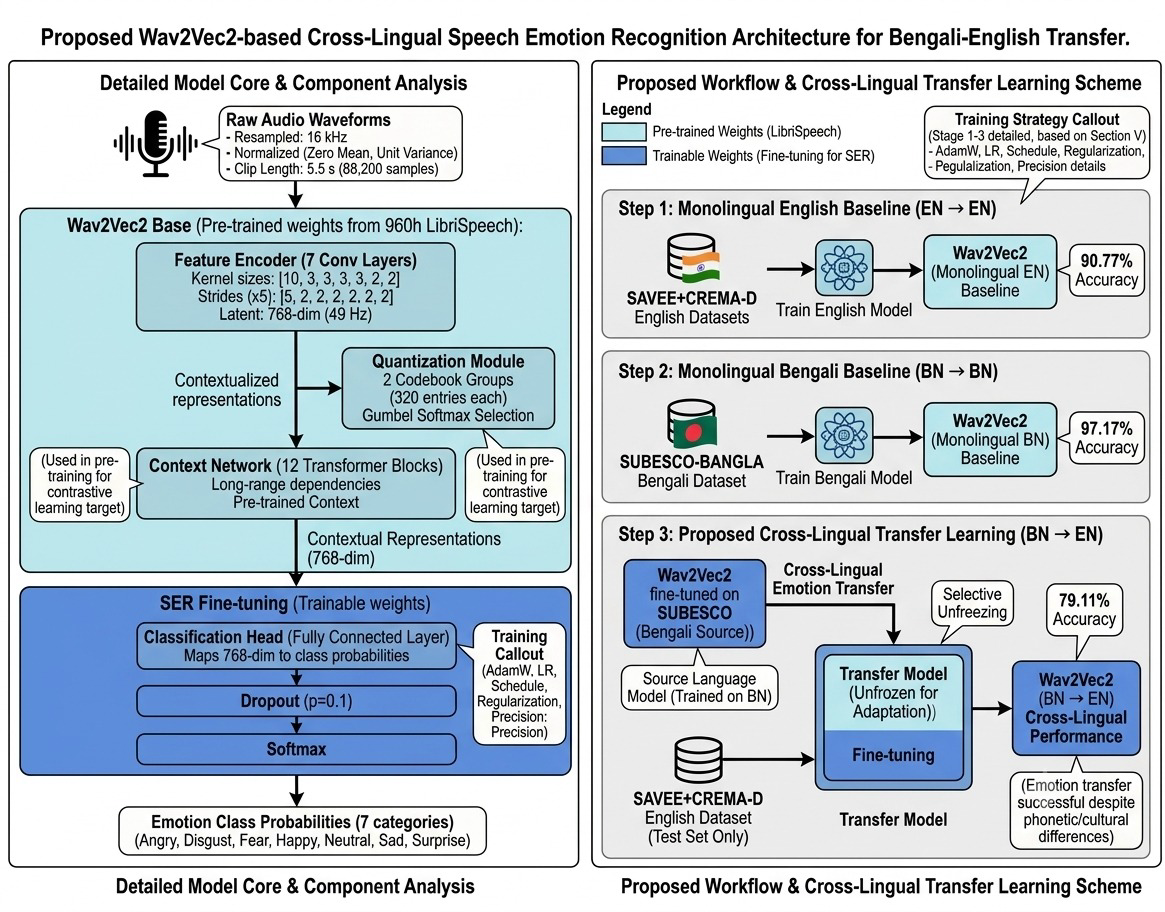
\includegraphics[width=\columnwidth]{fig8_architecture.png}
  \caption{Proposed Wav2Vec2-based Speech Emotion Recognition Architecture.}
  \label{fig:architecture}
\end{figure}

\subsection{Algorithm Description}

The overall training and workflow of the proposed cross-lingual Wav2Vec2-based Speech Emotion Recognition (SER) framework is summarized in Algorithm~\ref{alg:crosslingual_wav2vec2_ser}. The algorithm describes the complete processing pipeline, beginning with speech pre-processing, then the initialization and fine-tuning of the pre-trained Wav2Vec2 model, and concluding with emotion prediction and performance evaluation under monolingual and cross-lingual experimental settings. The required input datasets, model parameters, intermediate notations, and output evaluation metrics used throughout the algorithm are summarized in Table~\ref{tab:algorithm_notation}.

\begin{algorithm}[t]
...
\end{algorithm}

\begin{table}[t]
...
\end{table}

%% ============================================================
%%  7. DATABASE DESCRIPTION
%% ============================================================
\section{Database Description}

\noindent\textbf{1.\enspace SAVEE (Surrey Audio-Visual Expressed Emotion) Database~\cite{haq2009}.}
This dataset features the speech of four native British-English males aged between 27 and 31
years covering seven emotional classes. It consists of 480 utterances of 15 TIMIT sentences
plus 30 additional phrases, all recorded in a controlled studio environment at 44.1~kHz.
Strengths include high-quality recordings and clear emotional expression; limitations include
a small pool of only male speakers, acted emotions and limited accent diversity.

\smallskip
\noindent\textbf{2.\enspace CREMA-D (Crowd-Sourced Emotional Multimodal Actors Dataset)~\cite{cao2014}.}
Comprising American English voice recordings from 91 actors (48 male, 43 female) aged
20--74, this dataset has balanced ethnic representation across six emotions (excluding
Surprise). The clips have different emotional intensity levels and are captured at a 16~kHz sampling rate. The strength is speaker diversity and crowd validated labels. It has some limitations that is it includes acted emotions.

\smallskip
\noindent\textbf{3.\enspace SUBESCO-BANGLA (Bengali Emotional Speech Corpus)~\cite{rahman2019}.}
This data set is of Bengali native recording in Bangladesh and West.
Bengal, India. It has seven emotions which were captured at 16 kHz on a professional equipment. The data represents domestic emotional dissimilar manifestations offering culturally related background though is smaller than its counterpart, which is English data and the occurrence of acted emotions.

\smallskip
\noindent\textbf{Data Pre-processing Pipeline:}
\begin{itemize}
  \item \textit{Resampling:} Resampled all audio files to 16 kHz so that they can be used by Wav2Vec2.
  \item \textit{Duration Normalization:} Duration Standard Clip length is 5.5s; Longer clips are fert clips trimmed and short clips are zero padded.
  \item \textit{Amplitude Normalization:} This is a method that guarantees the same volume of records through peak normalization.
  \item \textit{Channel Conversion:} Two-track audio can be transformed into single-track audio.
  \item \textit{Augmentation:} 10\% of the time filling is between 0.98 1.02 to lesser imitation of the natural language variants with an emotional touch, without shifting of the pitch or addition of noise.
\end{itemize}

%% ============================================================
%%  8. RESULTS AND ANALYSIS
%% ============================================================
\section{Results and Analysis}
\subsection{Monolingual English Emotion Recognition
  (EN\,$\rightarrow$\,EN): 90.77\%}
Obtained 90.77\% accuracy using the model that was trained on the category of SAVEE and CREMA-D datasets. The model was trained over 16 epoch sizes of 8 batch size which leads to the effective 16 batch size running in about 2 hours.

\noindent\textbf{Performance Metrics:}
\begin{itemize}
  \item Overall Test Accuracy: 90.77\%
  \item Training Accuracy: 93.42\% (indicating slight overfitting)
  \item Precision (macro-averaged): 0.9082
  \item Recall (macro-averaged): 0.9077
  \item F1-Score (macro-averaged): 0.9075
\end{itemize}

\begin{figure}[htbp]
  \centering
  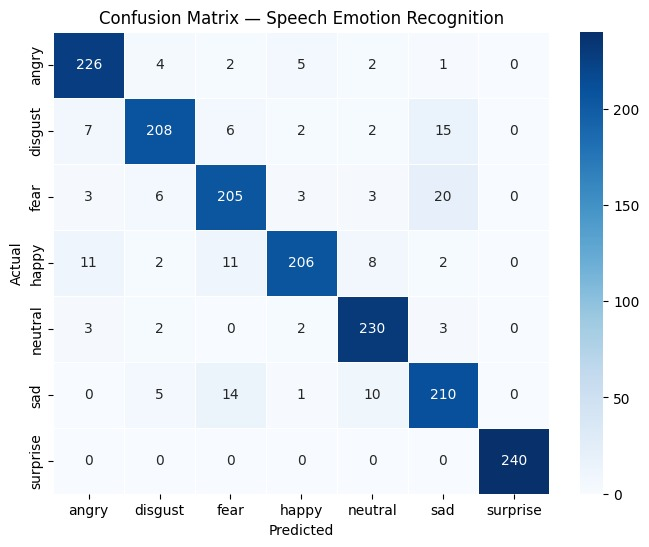
\includegraphics[width=0.95\columnwidth]{fig1_en_confusion_matrix.png}
  \caption{EN\,$\rightarrow$\,EN Confusion Matrix.}
  \label{fig:en_cm}
\end{figure}

\begin{figure}[htbp]
  \centering
  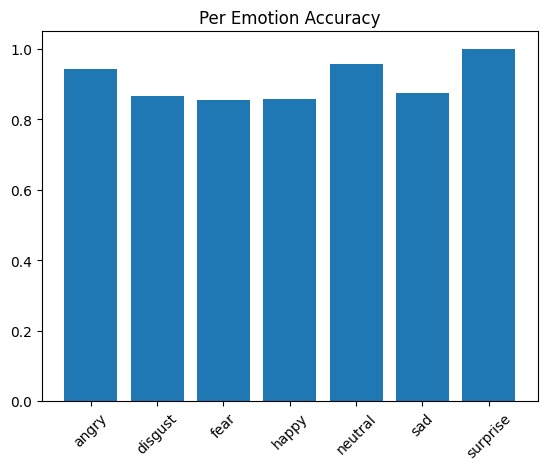
\includegraphics[width=0.95\columnwidth]{fig2_en_per_emotion_accuracy.png}
  \caption{EN\,$\rightarrow$\,EN Per Emotion Accuracy.}
  \label{fig:en_acc}
\end{figure}

\noindent\textbf{Key Observations:}
\begin{itemize}
  \item \textit{Confusion Patterns:} The model shows confusion between emotions
        with same type of arousal levels.
  \item \textit{Training Dynamics:} Gradual refinement is done in epochs 6--15, with
        stabilization in epochs 16--20 showing minimal improvement.
  \item \textit{Dataset Synergy:} Combining datasets improved performance by providing
        diverse emotional expressions and speaker characteristics.
\end{itemize}

\subsection{Monolingual Bengali Emotion Recognition
  (BN\,$\rightarrow$\,BN): 97.17\%}

Training only on the SUBESCO-BANGLA dataset achieved a remarkable 97.17\% accuracy,
that is 6.4\% higher than the English model. The training has taken 12 epochs.

\noindent\textbf{Performance Metrics:}
\begin{itemize}
  \item Overall Test Accuracy: 97.17\%
  \item Training Accuracy: 98.23\%
  \item Precision (macro-averaged): 0.9721
  \item Recall (macro-averaged): 0.9717
  \item F1-Score (macro-averaged): 0.9718
\end{itemize}

\begin{figure}[htbp]
  \centering
  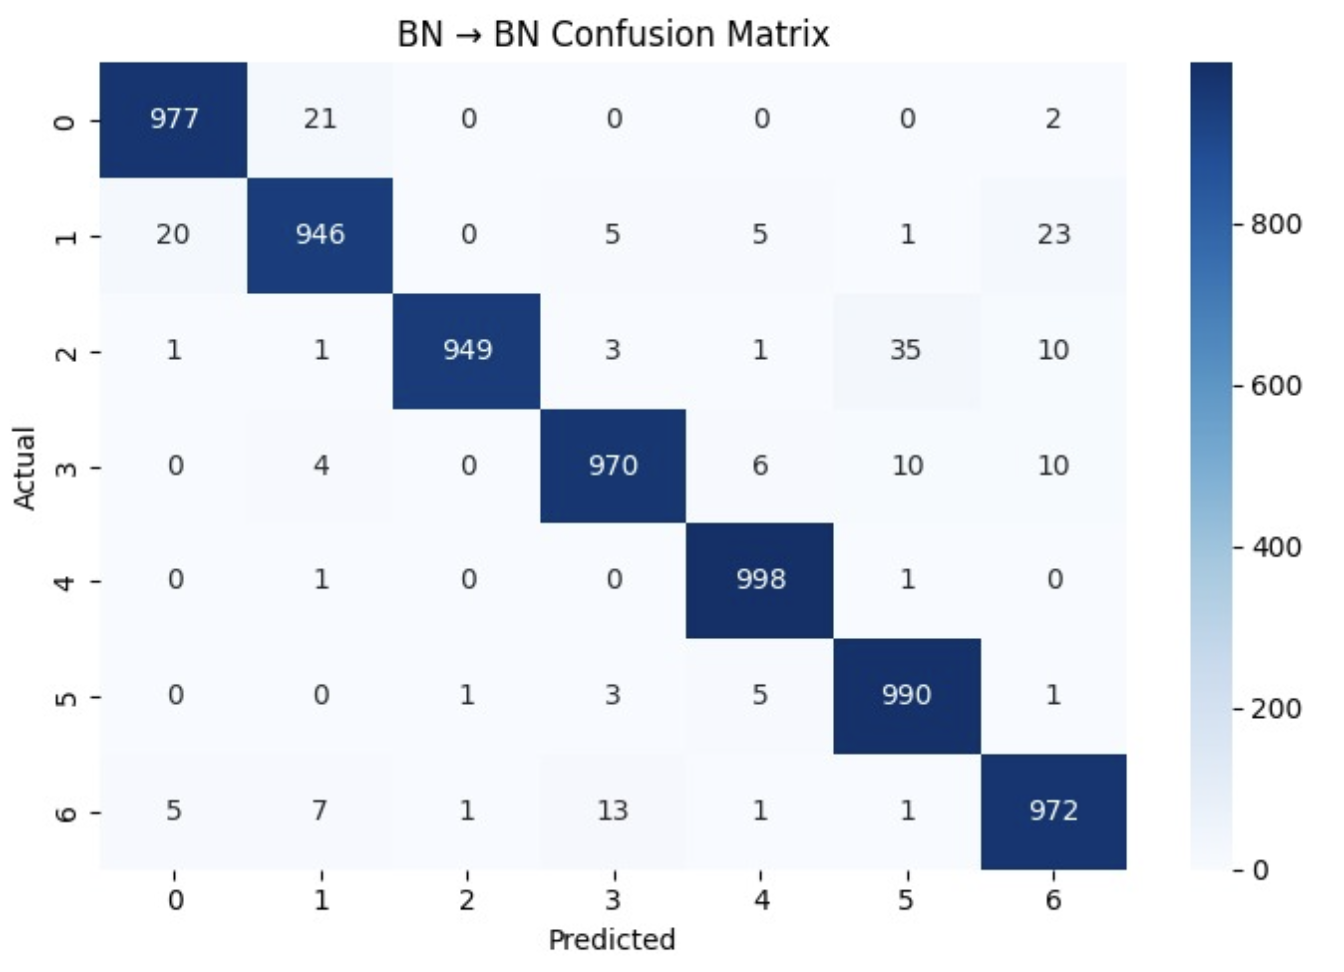
\includegraphics[width=0.95\columnwidth]
  {fig3_bn_confusion_matrix.png}
  \caption{BN\,$\rightarrow$\,BN Confusion Matrix.}
  \label{fig:bn_acc}
\end{figure}

\begin{figure}[htbp]
  \centering
  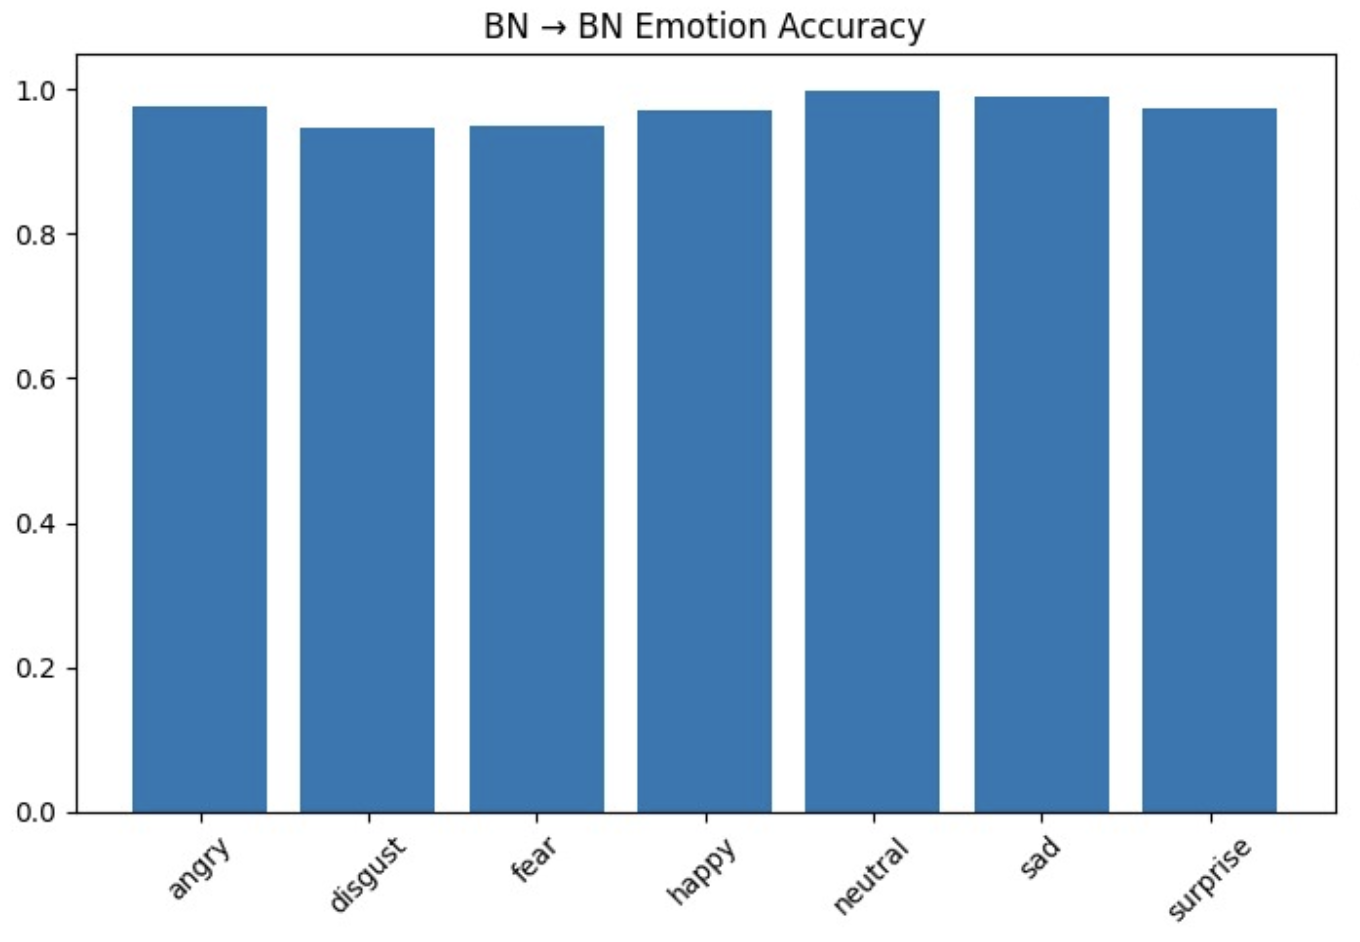
\includegraphics[width=0.95\columnwidth]{fig4_bn_per_emotion_accuracy.png}
  \caption{BN\,$\rightarrow$\,BN Per Emotion Accuracy.}
  \label{fig:bn_cm}
\end{figure}

\noindent\textbf{Factors Contributing to Superior Performance:}
\begin{itemize}
  \item More consistent recording conditions resulted in clearer emotional expressions.
  \item Bengali's distinct patterns enhanced emotion expression.
  \item The Wav2Vec2 model capacity is well suited for the dataset.
\end{itemize}

\subsection{Cross-Lingual Transfer
  (Bengali\,$\rightarrow$\,English): 79.11\%}

This approach achieved 79.11\% accuracy, showing that the transfer of emotion
recognition is meaningful despite linguistic differences. The training was done with 10 epochs with a reduced
learning rate of $5{\times}10^{-6}$.

\noindent\textbf{Performance Metrics:}
\begin{itemize}
  \item Overall Test Accuracy: 79.11\%
  \item Degradation from English Monolingual: 11.66\%
  \item Precision (macro-averaged): 0.7823
  \item Recall (macro-averaged): 0.7911
  \item F1-Score (macro-averaged): 0.7856
\end{itemize}

\begin{figure}[htbp]
  \centering
  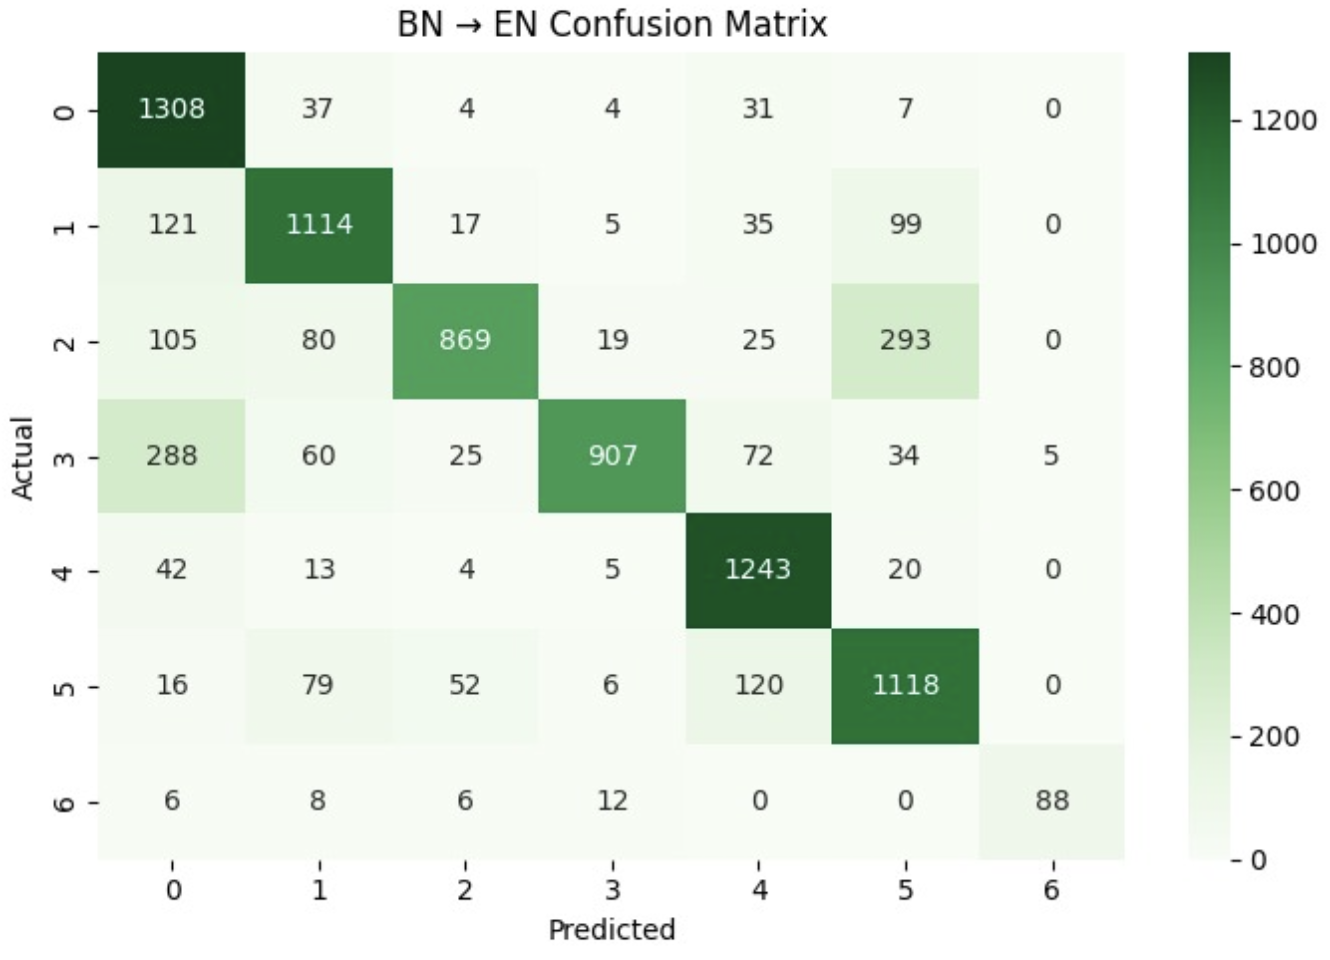
\includegraphics[width=0.95\columnwidth]{fig5_bnen_confusion_matrix.png}
  \caption{BN\,$\rightarrow$\,EN Confusion Matrix.}
  \label{fig:bnen_cm}
\end{figure}

\begin{figure}[htbp]
  \centering
  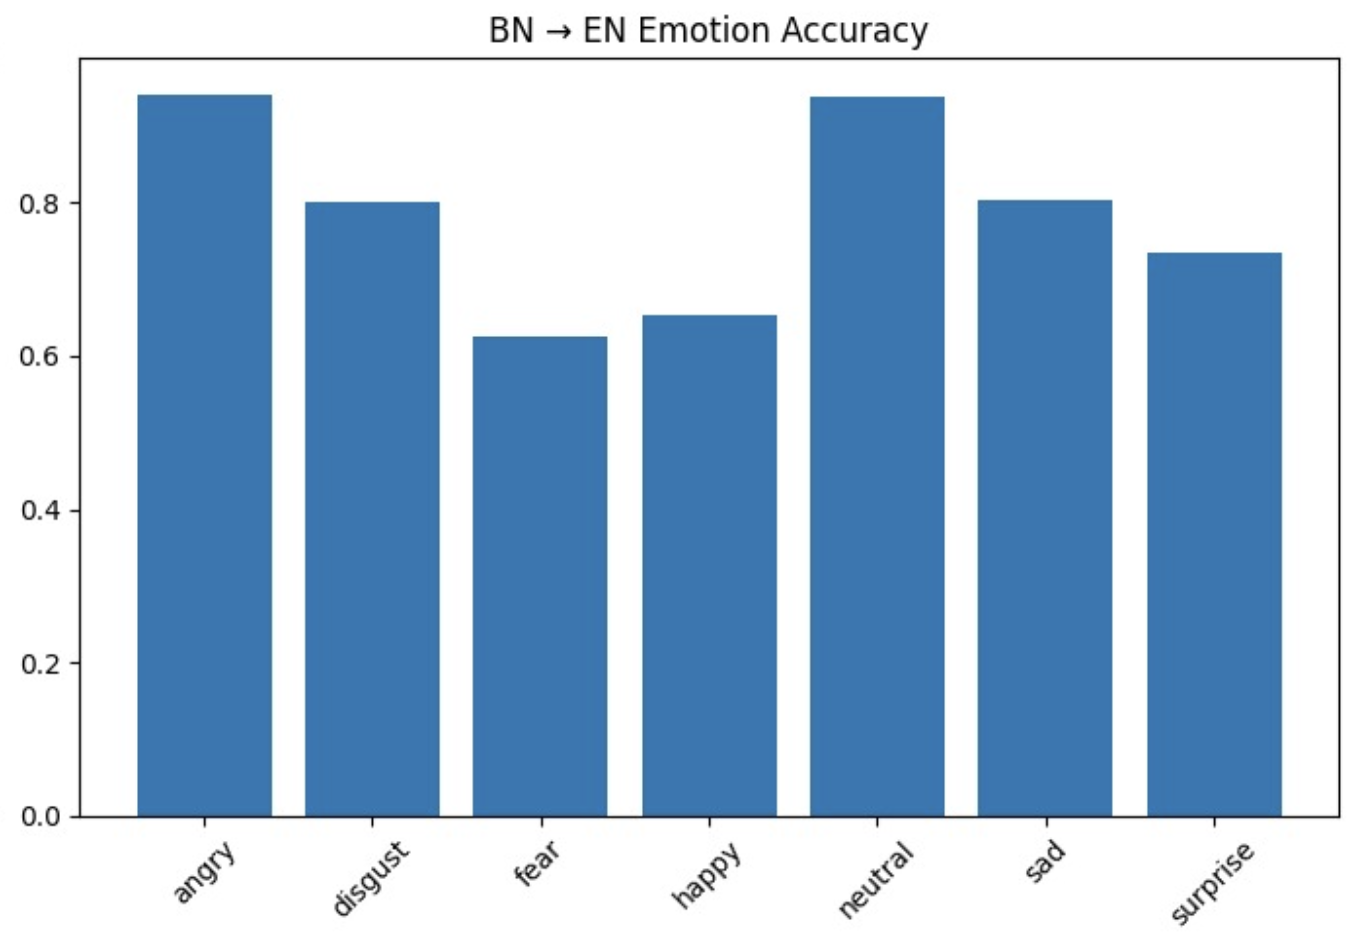
\includegraphics[width=0.95\columnwidth]{fig6_bnen_per_emotion_accuracy.png}
  \caption{BN\,$\rightarrow$\,EN Per Emotion Accuracy.}
  \label{fig:bnen_acc}
\end{figure}

\noindent\textbf{Comparison to Random Baseline:}
The model's performance significantly exceeded random guessing, which had got about
14.29\% accuracy.

\smallskip
\noindent\textbf{Cross-Lingual Confusion Patterns:}
Misclassifications are there, particularly between low-arousal negative emotions and high-arousal
positive ones.

%% ============================================================
%%  9. MODEL COMPARISON AND QUANTITATIVE ANALYSIS
%% ============================================================
\section{Model Comparison and Quantitative Analysis}

Table~\ref{tab:model_comparison} provides a quantitative comparison of the different model
configurations, and Fig.~\ref{fig:model_acc} shows the corresponding accuracy comparison chart.

\begin{figure}[htbp]
  \centering
  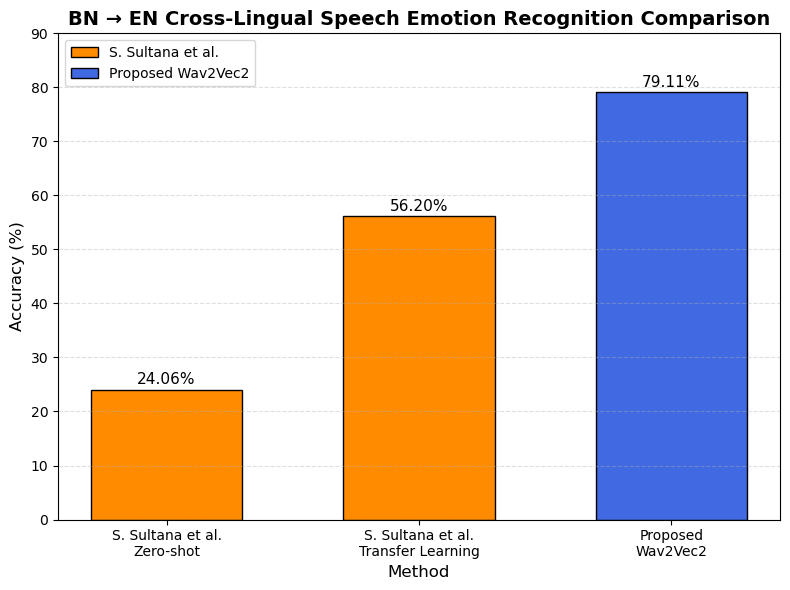
\includegraphics[width=0.95\columnwidth]{fig7_model_accuracy_comparison.png}
  \caption{Model Accuracy Comparison
    (S. Sultana et as. zero shot, S. Sultana et al Transfer Learning Method, Proposed Wav2Vec2)}
  \label{fig:model_acc}
\end{figure}

%% ── Table I: Model Comparison ──────────────────────────────
\begin{table}[htbp]
\caption{Comparison of Bengali-to-English (BN$\rightarrow$EN) cross-lingual speech emotion recognition performance.}
\label{tab:crosslingual_comparison}
\centering
\begin{tabular}{@{}lcc@{}}
\toprule
\textbf{Method} & \textbf{Training Strategy} & \textbf{Accuracy (\%)} \\
\midrule
S. Sultana et al. (DCTFB) &
Cross-corpus (Zero-shot) &
24.06 (WA) \\

S. Sultana et al. (DCTFB) &
Transfer Learning (Fine-tuning) &
56.20 (WA) \\

\textbf{Proposed Wav2Vec2} &
Cross-lingual (BN$\rightarrow$EN) &
\textbf{79.11} \\
\bottomrule
\end{tabular}
\end{table}

\subsection{Comparison Analysis}
Table~\ref{tab:crosslingual_comparison} presents a comparison of the our proposed Wav2Vec2-based cross-lingual speech emotion recognition model with the approach reported by S.~Sultana \textit{et al.}~\cite{sultana2022} for the Bengali-to-English (BN$\rightarrow$EN) task. In the zero-shot cross-corpus setting, the best-performing DCTFB model scored a weighted accuracy (WA) of 24.06\%, on the other hand the proposed model achieved an overall accuracy of 79.11\%, corresponding to an improvement of 55.05 percentage points. Further, compared with the transfer learning (fine-tuning) approach in~\cite{sultana2022}, which achieved a WA of 56.20\%, the proposed model still has an absolute improvement of 22.91 percentage points. These results show that the self-supervised Wav2Vec2 architecture learns more robust and transferable speech representations, enabling much better cross-lingual emotion recognition performance than conventional CNN-BLSTM-based methods.

%% ============================================================
%%  10. DISCUSSION AND ANALYSIS
%% ============================================================
\section{Discussion and Analysis}

Effectiveness of Wav2Vec2 is proved by high-performance among models and in particular - Bengali recognition. There is a lot of emotion in cross-lingual accuracy
transferred under some phonetic and cultural difficulties. The study highlights the need of the continuous improvements, especially in phonetics alignment and modelling of the emotional expression.

\smallskip
\noindent\textbf{Challenges:}
\begin{itemize}
  \item The latent of computer power demanded the careful method.
  \item Issues of data were correct emotion matching and class balancing.
  \item Language barriers were a serious issue that had to be carefully addressed when designing the models.
\end{itemize}

\noindent\textbf{Challenges and Technologies:}
\begin{itemize}
  \item \textit{Computational:} FP16 precision was necessary due to memory concerns, gradient accumulation and good data loading; Tuning of hyperparameters based on balanced transfer-learning and adaptation.
Data: There was a need to integrate data in terms of emotion alignment, resampling to 16 kHz and class balancing; Duration normalized balanced information content and efficiency.
Linguistic: Phonetic alignment problems, prosodic transfer problems and diversity in the expression of culture had to be modeled carefully.

  \item \textit{Data:} Dataset integration required emotion alignment, resampling to 16~kHz
        and class balancing; duration normalization (5.5~s) balanced information content and
        efficiency.
  \item \textit{Linguistic:} Phonetic alignment challenges, prosodic transfer difficulties and
        cultural expression variations required careful model design.
  \item \textit{Technologies:} PyTorch 1.12+, Transformers 4.25+, LIBROSA 0.9+,
        CUDA~11.6, Matplotlib/Seaborn.
\end{itemize}

%% ============================================================
%%  CONCLUSION
%% ============================================================
\section*{Conclusion}

The research will offer reference points to Bengali-English SER by utilizing Wav2Vec2 with significant accuracies. It presents opportunities of further investigations of the multidimensional language comprehension and emotional expression optimization across
dissimilar language sceneries.

%% ============================================================
%%  REFERENCES  (IEEE numbered style)
%% ============================================================
\begin{thebibliography}{25}

\bibitem{sultana2022}
S.~Sultana, M.~Z.~Iqbal, M.~R.~Selim, Md.~M.~Rashid, and M.~S.~Rahman,
``Bangla Speech Emotion Recognition and Cross-Lingual Study Using Deep CNN and BLSTM Networks,''
\textit{IEEE Access}, vol.~10, pp.~564--578, 2022.

\bibitem{bhattacharya2024}
S.~Bhattacharya, B.~K.~Mishra, S.~Borah, N.~Das, and N.~Dey,
``Cross-lingual Deep Learning Model for Gender-Based Emotion Detection,''
\textit{Multimedia Tools and Applications}, vol.~83, no.~9, pp.~25969--26007, 2024.

\bibitem{bhattacharya2023}
S.~Bhattacharya, B.~K.~Mishra, and S.~Borah,
``Multilingual and Cross Lingual Audio Emotion Analysis Using RNN,''
in \textit{Advances in IoT and Security with Computational Intelligence},
Lecture Notes in Networks and Systems, Springer, Singapore,
pp.~171--188, 2023.

\bibitem{baevski2020}
A.~Baevski et al.,
``wav2vec 2.0: Framework for Self-Supervised Learning,''
\textit{NeurIPS}, vol.~33, pp.~12449--12460, 2020.

\bibitem{ekman1992}
P.~Ekman,
``Argument for Basic Emotions,''
\textit{Cognition \& Emotion}, vol.~6, no.~3--4, pp.~169--200, 1992.

\bibitem{haq2009}
S.~Haq and P.~Jackson,
``Speaker-dependent Audio-visual Emotion Recognition,''
\textit{AVSP}, pp.~53--58, 2009.

\bibitem{cao2014}
H.~Cao et al.,
``CREMA-D Dataset,''
\textit{IEEE TAC}, vol.~5, no.~4, pp.~377--390, 2014.

\bibitem{rahman2019}
M.~Rahman et al.,
``SUBESCO: Bangla Emotional Speech Corpus,''
\textit{Proc.\ Bangla Speech}, pp.~85--90, 2019.

\bibitem{trigeorgis2016}
G.~Trigeorgis et al.,
``End-to-End Speech Emotion Recognition,''
\textit{ICASSP}, pp.~5200--5204, 2016.

\bibitem{mirsamadi2017}
S.~Mirsamadi et al.,
``Automatic SER Using RNNs,''
\textit{ICASSP}, pp.~2227--2231, 2017.

\bibitem{chen2018}
M.~Chen et al.,
``3-D Convolutional RNNs,''
\textit{IEEE SPL}, vol.~25, no.~10, pp.~1440--1444, 2018.

\bibitem{huang2021}
Y.~Huang et al.,
``Cross-Lingual SER Using Transfer Learning,''
\textit{INTERSPEECH}, pp.~4189--4193, 2021.

\bibitem{schneider2019}
W.~Schneider et al.,
``wav2vec: Unsupervised Pre-training,''
\textit{INTERSPEECH}, pp.~3465--3469, 2019.

\bibitem{chung2019}
Y.-A.~Chung et al.,
``Unsupervised Autoregressive Model,''
\textit{INTERSPEECH}, pp.~146--150, 2019.

\bibitem{riviere2020}
G.~Rivi\`{e}re et al.,
``Unsupervised Pretraining Transfer,''
\textit{ICASSP}, pp.~7414--7418, 2020.

\bibitem{busso2008}
C.~Busso et al.,
``IEMOCAP Database,''
\textit{Language Resources and Evaluation}, vol.~42, no.~4, pp.~335--359, 2008.

\bibitem{burkhardt2005}
F.~Burkhardt et al.,
``Database of German Emotional Speech,''
\textit{INTERSPEECH}, pp.~1517--1520, 2005.

\bibitem{livingstone2018}
S.~Livingstone and F.~Russo,
``RAVDESS Dataset,''
\textit{PLoS ONE}, vol.~13, no.~5, e0196391, 2018.

\bibitem{aldeneh2017}
Z.~Aldeneh and E.~Provost,
``Using Regional Saliency,''
\textit{ICASSP}, pp.~2741--2745, 2017.

\bibitem{devlin2019}
J.~Devlin et al.,
``BERT Pre-training,''
\textit{NAACL-HLT}, pp.~4171--4186, 2019.

\bibitem{vaswani2017}
A.~Vaswani et al.,
``Attention is All You Need,''
\textit{NeurIPS}, vol.~30, pp.~5998--6008, 2017.

\bibitem{hochreiter1997}
S.~Hochreiter and J.~Schmidhuber,
``LSTM,''
\textit{Neural Computation}, vol.~9, no.~8, pp.~1735--1780, 1997.

\bibitem{lecun2015}
Y.~LeCun et al.,
``Deep Learning,''
\textit{Nature}, vol.~521, pp.~436--444, 2015.

\bibitem{han2014}
K.~Han et al.,
``SER Using DNN,''
\textit{INTERSPEECH}, pp.~223--227, 2014.

\bibitem{deng2013}
J.~Deng et al.,
``Sparse Autoencoder Feature Transfer,''
\textit{ACII}, pp.~511--516, 2013.

\bibitem{elayadi2011}
M.~El~Ayadi et al.,
``Survey on SER,''
\textit{Pattern Recognition}, vol.~44, no.~3, pp.~572--587, 2011.

\bibitem{lee2005}
C.~Lee and S.~Narayanan,
``Detecting Emotions in Dialogs,''
\textit{IEEE TSAP}, vol.~13, no.~2, pp.~293--303, 2005.

\end{thebibliography}

\end{document}